\section{Matrizen}
\subsection{Hermitesche Matrizen}
\begin{itemize}
    \item $\iff A^H = A$
    \item $\implies$ Eigenwerte $\lambda_i \in \mathbb{R}$
    \item $\implies A$ normal
    \item $\implies$ unitär diagonalisierbar. 
\end{itemize}

\subsection{Invertierbare/Reguläre Matrizen}
\begin{itemize}
    \item $\iff \det{A} \neq 0$ 
\end{itemize}

\subsection{Unitäre Matrizen}
\begin{itemize}
    \item $\iff A^H = A^{-1}$
    \item $\implies A$ regulär ($\iff$ invertierbar)
    \item $\implies |\det{A}| = 1$
    \item $\implies A$ normal
    \item $\implies$ Eigenvektoren orthonormal
\end{itemize} 

\subsection{Normale Matrizen}
\begin{itemize}
    \item $\iff A^H A = A A^H$
    \item $\iff A$ unitär diagonalisierbar
\end{itemize}

\subsection{Diagonalisierbare Matrizen}
\begin{itemize}
    \item $\iff S^{-1}AS = D$, $D$ Diagonalmatrix
\end{itemize}
\subsubsection{Diagonalisierbarkeit zeigen}
\begin{itemize}
    \item Charakteristisches Polynom zerfällt in Linearfaktoren
    \item $\wedge$ Geometrische und Algebraische Vielfachheiten stimmen überein
\end{itemize}

\subsubsection{Unitär Diagonalisierbare Matrizen}
\begin{itemize}
    \item $\iff \exists S$ unitär $\mid S^H=S^{-1}$
    \item $\implies$ Eigenvektoren orthogonal
\end{itemize}

\subsection{Spur einer Matrix}
Die Spur einer Matrix A ist die Summe der Hauptdiagonalelemente\\ $\sum\nolimits_{i=1}^n a_{ii} = Spur(A)$.
\begin{itemize}
    \item bei diagonalisierbaren Matrizen ist die Spur die Summe der Eigenwerte $\implies$ die Spur ähnlicher Matrizen ist gleich
    \item die Spur ist eine lineare Abbildung
    \item Vertauschung unter der Spur: $Spur(AB)=Spur(BA)$
    \item Invarianz bei zyklischen Vertauschungen $Spur(ABC)=Spur(BCA)=Spur(CAB)$
\end{itemize}

\subsection{Diagonalisieren von Matrizen}
Matrix $A$ diagonalisierbar $\iff D_A=S^{-1}AS$, $A=SDS^{-1}$. Es sollen $D_A$ und $S$ berechnet werden.
\begin{enumerate}
    \item Bestimmen der Eigenwerte $\lambda_i$ mittels $\det(A-\lambda I) = 0$.
    \item Bestimmen der Eigenräume $E(\lambda_i)$ zu den Eigenwerten mittels $(A-\lambda_iI)\cdot x = 0$
    \item Bestimmen der Basisvektoren $b$ der Eigenräume
    \item $D_A = \text{diag}(\lambda_1,\dots , \lambda_n)$\\ $S=(b_1,\dots,b_n)$
\end{enumerate}

\subsection{Definitheit}
Wenn eine Matrix nicht symmetrisch oder hermitesch ist, kann nur der symmetrische oder
hermitesche Teil betrachtet werden: $A_S=\frac{1}{2} (A+A^T)$ bzw $A_H=\frac{1}{2}(A+A^H)$.

\subsubsection{Definition}
Eine Matrix ist genau dann\\
\begin{tabular}{l l}
    positiv definit,	    &falls $x^{T}Ax>0$\\
    positiv semidefinit,	&falls  $x^{T}Ax\geq 0$\\
    negativ definit,	    &falls  $x^{T}Ax<0$\\
    negativ semidefinit,	&falls  $x^{T}Ax\leq 0$.
\end{tabular}

\subsubsection{Definitheit anhand von Eigenwerten}
Eine Matrix ist genau dann\\
\begin{tabular}{l l}
    positiv definit,        &wenn alle Eigenwerte größer als null sind;\\
    positiv semidefinit,	&wenn alle Eigenwerte größer oder gleich null sind;\\
    negativ definit,        &wenn alle Eigenwerte kleiner als null sind;\\
    negativ semidefinit,	&wenn alle Eigenwerte kleiner oder gleich null sind;\\
    indefinit,	            &wenn positive und negative Eigenwerte existieren.
\end{tabular}

\subsubsection{Definitheit anhand von Hauptminoren}
Positiv definit: Führende Hauptminoren sind positiv\\
Negativ definit: Vorzeichen der führenden Hauptminoren alternieren
(ungerade führende Hauptminoren negativ, alle geraden positiv).

\subsection{Satz von Cayley-Hamilton}
Matrix ist Nullstelle des Zugehörigen charakteristischen Polynoms:\\
$P_A(A) = (-1)^n(A^n + a_{n-1}A^{n-1}+\dots+a_0E_n)=0$\\
Durch Multiplizieren von $A^{-1}$ lässt sich damit $A^{-1}$ bestimmen.

% \section{Hauptachsentransformation}
% WORK IN PROGRESS/PLEASE FIX
% Gegeben sei Eine Quadrik $Q(x)=x^TAx+b^Tx+c=0$.
% Eventuell müssen die Matrizen noch aus einer gegebenen Gleichung aufgestellt werden.

% \begin{enumerate}
%     \item Bestimmen der Eigenwerte $\lambda_i$ von $A$ mittels $\det(A-\lambda I) = 0$.
%     \item Bestimmen der Eigenvektoren $e_i$ mit $(A-\lambda_i)\cdot e_i=0$ und anschließendem Normieren.
%     \item Aufstellen der Matrix $S=(e_1,\dots,e_n)$
%     \item Substituieren von $x,y,z$ durch $\widetilde{x},\widetilde{y},\widetilde{z}$ mit $(x,y,z)^T=S \cdot (\widetilde{x},\widetilde{y},\widetilde{z})^T$
% \end{enumerate}

\section{Determinanten}
\subsection{Umfomungen von Determinanten}
\begin{enumerate}
    \item \emph{Vertauschen} von Zeile oder Spalte $\implies$ Faktor $-1$ vor Determinante
    \item \emph{Multiplizieren} von Zeile $\implies$ Faktor vor Determinante
    \item \emph{Gauß} ohne Folgen
    \item $\det(A^{-1})=(\det(A))^{-1}$
\end{enumerate}

\section{Basiswechsel}
Ein VR zur Basis $A$ soll durch die Transformationsmatrix in die Basis $B$ umgeformt werden.
Berechnung der Trafomatrix mittels Gauß-Jodan:\\
$(B\mid A) \text{(Umformungen mit Gauß)} \implies  (E\mid T)$ \\ mit $E$ als Einheitsmatrix und $T$ als Tranformationsmatrix.
\subsection{Lineare Abbildung nach Basiswechsel}

Wichtig: Transformationsschritte links anmultiplizieren.

\begin{figure}[H]
    \centering
    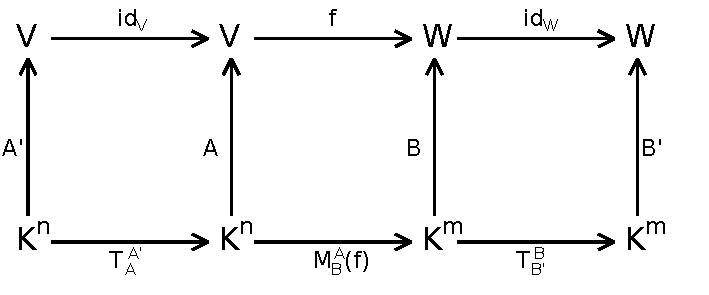
\includegraphics[width=0.8\textwidth]{Change_of_basis2.pdf}
    \caption{Basiswechsel linearer Abbildungen}
\end{figure}

In den meisten Fällen gilt bei uns $A=B$ und $ A'=B'$ und somit $T_{B'}^{B}$ invers zu $T_A^{A'}$. 

\section{Skalarprodukte}
Ein Skalarprodukt ist gegeben durch $f(x,y)= _{\dots} =x^T My$
\begin{enumerate}
    \item $\iff M$ hermitesch $\wedge$ $M$ positiv definit $\wedge$ M linear.
\end{enumerate}

\section{Lineare Abbildungen}
\subsection{Linearität zeigen}
\begin{itemize}
    \item Abbildung als Matrix darstellen
    \item $\alpha Lv = L(\alpha v) \wedge Lv_1 + Lv_2 = L(v_1+v_2)$
\end{itemize}

\subsection{Linearität widerlegen}
\begin{itemize}
    \item Additivität widerlegen: $Lv_1 + Lv_2 \neq L(v_1+v_2)$
    \item Abbildung auf Null widerlegen: $L0 \neq 0$
    \item Skalarmultiplikation widerlegen: $\alpha L v_1 \neq L(\alpha v_1)$
\end{itemize}


\section{Gram Schmidt}
\begin{enumerate}
    \item $u_1 = \frac{v_1}{\norm{v_1}}$
    \item $u_2^\prime = v_2 - \langle v_2,u_1 \rangle u_1$
    \item $u_2 = \frac{u_2^\prime}{\norm{u_2^\prime}}$
    \item $u_k^\prime = v_k - \sum_{i=1}^{k-1}\langle v_k,u_i\rangle u_i$
    \item $u_k = \frac{u_k^\prime}{\norm{u_k^\prime}}$
\end{enumerate}

\section{Vektorräume}
\subsection{Voraussetzungen}
\begin{itemize}
    \item $V \neq \varnothing$
    \item $(V,+)$ abelsche Gruppe (kommutative Vektoraddition)
        \begin{itemize}
            \item Assoziativität, Neutrales, Inverses, Kommutativität
        \end{itemize}
    \item \emph{Vektorraumaxiome}
        \begin{itemize}
            \item $1 \cdot v = v$
                \item $(\lambda + \mu)\cdot v = \lambda v + \mu v$,  $\lambda (v + w) = \lambda v + \lambda w$ Distributivgesetzt bzgl. Skalarmultiplikation, Vektoraddition
            \item  $\lambda (\mu v) = (\lambda \cdot \mu) \cdot v$ Assoziativgesetz
        \end{itemize}
\end{itemize}

\subsection{Vektorraum zeigen}
Einfacher als Axiome: \emph{Unterraumkriterium}:
\begin{itemize}
    \item Abgeschlossenheit bzgl. Vektoraddition
    \item Abgeschlossenheit bzgl. Skalarmultiplikation
\end{itemize}